\chapter{Phương pháp nghiên cứu}

\section{Kiến trúc tổng quát của hệ thống}
Để giải quyết các vấn đề đã được trình bày ở mục \ref{sec:muctieu},
hệ thống ứng dụng Chatbot tư vấn cần có ba module chính đó là phần
UI/UX giao tiếp với người dùng, phần nhập dữ liệu và phần lõi của hệ thống.

\begin{figure}[ht]
    \centering
    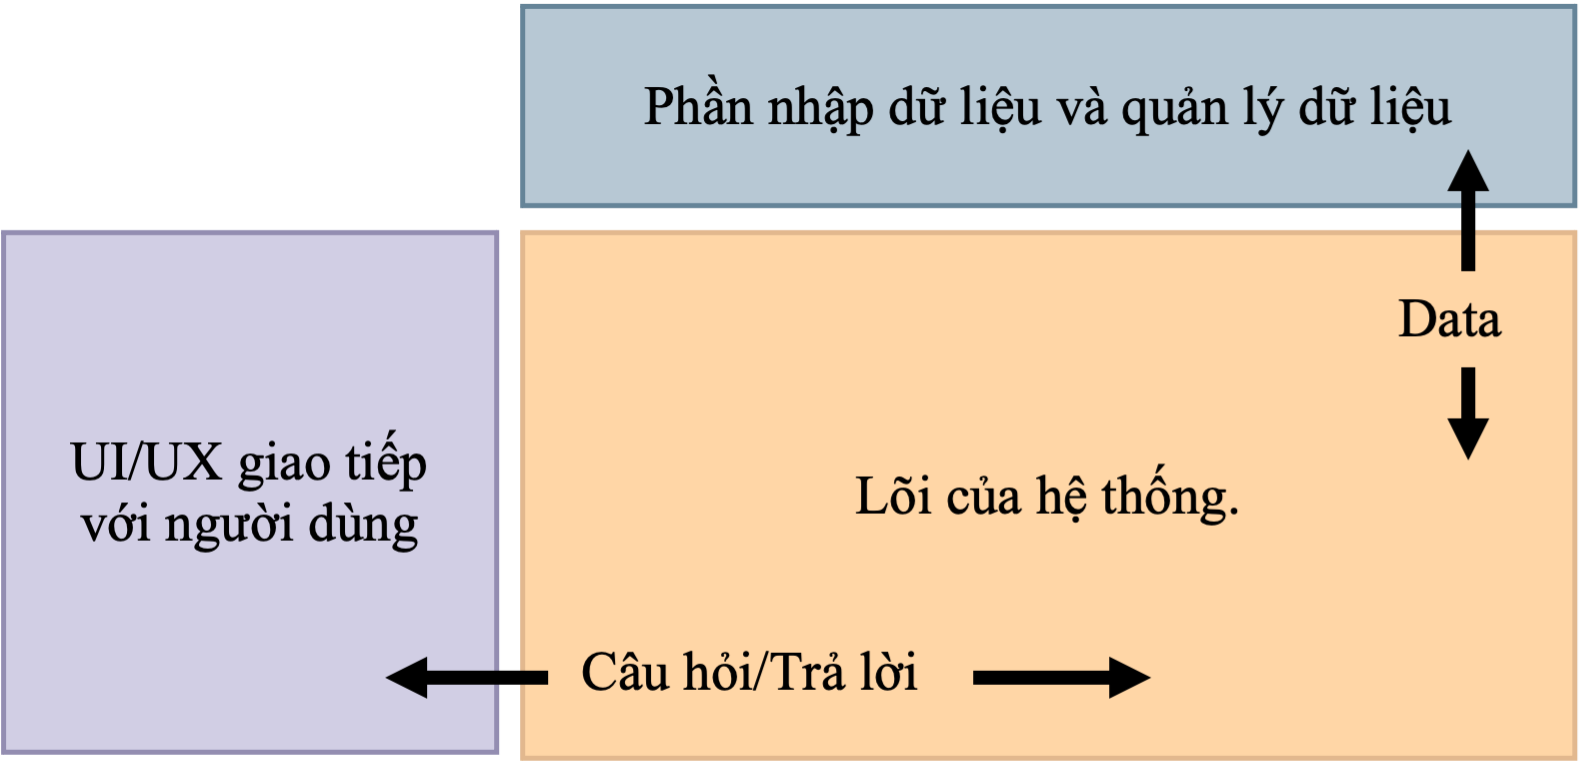
\includegraphics[width=1\textwidth]{thesis/chatbot-outline/phuongphap/chatbot_app.png}
    \caption{Kiến trúc tổng quát của ứng dụng Chatbot}
    \label{fig:chatbotapp}
\end{figure}

Trong phần lõi của hệ thống, ta có các phần con khác như mô tả
trong hình \ref{fig:chatbot}. Vì phạm vi của đề tài quá lớn nên
trong đề tài này, chỉ thực hiện phần huấn luyện cho agent sử dụng
phương pháp học tăng cường với mô hình Deep Q-Learning như được
mô tả ở mục \ref{sec:model}, đồng thời xây dựng bộ mô phỏng người dùng
và tạo lỗi để làm dữ liệu đầu vào cho việc huấn luyện mô hình.
Các thành phần còn lại sẽ được tích hợp vào một hệ thống Chatbot
có sẵn khác.

\section{Kiến trúc tổng quát của mô hình}
Đề tài áp dụng kiến trúc trong bài hướng dẫn \cite{traininggochatbot}
được mô tả như hình \ref{fig:agentmodel}, cũng như sẽ có một số
điều chỉnh để phù hợp với dữ liệu và yêu cầu của hệ thống sao cho
đáp ứng được lĩnh vực đang thực hiện.

\begin{figure}[ht]
    \centering
    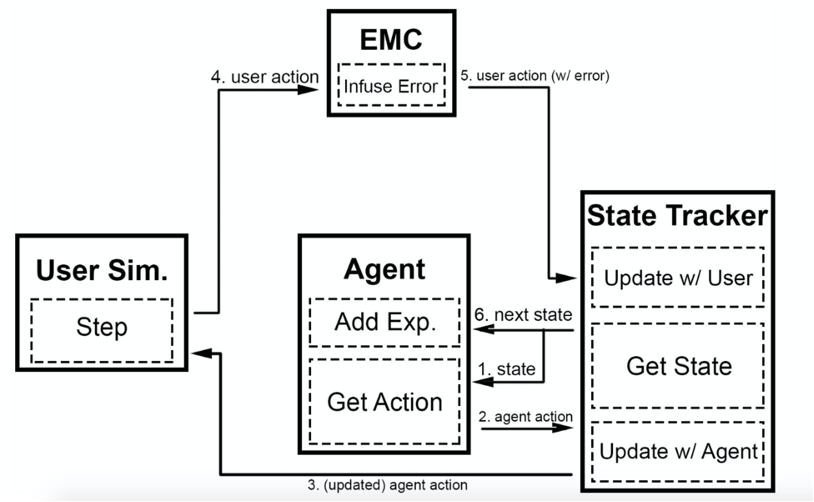
\includegraphics[width=1\textwidth]{thesis/chatbot-outline/phuongphap/agentmodel.png}
    \caption{Kiến trúc tổng quát của mô hình RL agent}
    \label{fig:agentmodel}
\end{figure}

Kiến trúc này mô tả một vòng huấn luyện sẽ được diễn ra. Cụ thể:

\begin{itemize}
    \item \textbf{Bước 1:} Lấy ra \textit{state} - trạng thái hiện tại
    từ \textit{dialog state tracker}, \textit{state} này có thể là
    \textit{state} khởi tạo nếu như vừa bắt đầu hội thoại hoặc là
    \textit{state} của toàn bộ cuộc hội thoại giữa user và Chatbot.
    \textit{State} sau khi được lấy ra sẽ làm input (đầu vào) cho
    \textit{agent} ở bước tiếp theo.
    \item \textbf{Bước 2:} \textit{Agent} sau khi nhận được input
    từ bước trước sẽ sinh ra \textit{action} (hành động) và gửi
    ngược về lại \textit{dialog state tracker}. \textit{Action}
    lúc này ở dạng thô, chưa kèm thông tin cụ thể. Nó sẽ được
    \textit{dialog state tracker} cập nhật thông tin sau khi thực hiện
    truy vấn lên cơ sở dữ liệu. Đồng thời \textit{dialog state tracker}
    cũng sẽ cập nhật lại trạng thái của hội thoại.
    \item \textbf{Bước 3:} \textit{Action} sau khi được cập nhật đầy đủ
    thông tin sẽ được gửi cho \textit{user simulator}.
    \textit{User simulator} sẽ dựa vào các luật đã được quy định trước
    để sinh ra \textit{action} (có cấu trúc tương tự \textit{action}
    của \textit{agent} ở bước trước), kèm theo \textit{reward} (điểm thưởng)
    và tín hiệu success (thành công) để giúp \textit{agent} có thể
    tự điều chỉnh hành vi để học.
    \item \textbf{Bước 4:} \textit{Action} của user ở bước trước đó
    sẽ được đưa qua \textit{EMC}, mục đích là tạo ra các lỗi mà
    user thật hay mắc phải, giúp \textit{agent} có hành vi chính xác
    và tự nhiên hơn khi chạy ở thực tế.
    \item \textbf{Bước 5:} \textit{Action} ở bước trước sẽ tiếp tục
    được gửi đi đến \textit{dialog state tracker} và được cập nhật
    thông tin cụ thể tương tự ở bước 2. Đồng thời
    \textit{dialog state tracker} cũng cập nhật trạng thái của nó.
    \item \textbf{Bước 6:} Trạng thái tiếp theo được lấy từ
    \textit{dialog state tracker} và quay lại giống bước 1.
\end{itemize}

\section{Bộ mô phỏng người dùng (User Simulator)}
Mục đích của \textit{User Simulator} là dùng để mô phỏng người dùng
thật để tương tác với \textit{agent} cũng như chấm điểm nó.
Việc này sẽ tốn rất nhiều thời gian nếu như làm với người thật.
Bộ \textit{User Simulator} này sẽ được hiện thực theo dạng
luật định sẵn. Cụ thể với mỗi lần tham gia cuộc hội thoại
(gọi là \textit{episode}), ta đều quy định sẵn các mục tiêu
(\textit{user goal}) và thực hiện các \textit{action} phù hợp với
mục tiêu đó, mỗi \textit{action} sẽ kèm theo các thông tin như
\textit{slot} mà nó sẽ \textit{request} hay \textit{inform}.

\textit{User goal} có thể có được từ các cuộc hội thoại thực hoặc
được làm thủ công (hoặc cả hai). Mỗi \textit{user goal} gồm các
\textit{inform slots} và \textit{request slots}.

Ví dụ, ta có một cuộc hội thoại sau đây:

\begin{verbatim}
Customer: [Hình ảnh sản phẩm] (mã sp là AT001)
Customer: Áo này có size XL không bạn?
Admin: Có bạn nha.
Customer: Có những màu nào nữa vậy bạn.
Admin: Mẫu áo AT001 này có 3 màu ạ. Đỏ, Trắng, Đen.
\end{verbatim}

Trong cuộc hội thoại, khách hàng yêu cầu số lượng và màu sắc của sản phẩm với mã sản phẩm và kích thước mà họ cung cấp. Từ đó, ta sẽ có một \textit{user goal} như sau:

\begin{lstlisting}[language=Python]
{
    "request_slots": {
        "amount": ["UNK"],
        "color": ["UNK"]
    },
    "inform_slots": {
        "name": ["AT001"],
        "size": ["XL"]
    }
}
\end{lstlisting}

Khi quá trình huấn luyện diễn ra, tại mỗi \textit{episode}, bộ
\textit{User Simulator} sẽ ngẫu nhiên chọn ra một \textit{user goal}
từ một danh sách và sẽ lần lượt gửi các \textit{action} tương ứng
phù hợp với \textit{user goal} đã được chọn tới \textit{agent}.

Để làm được điều trên, bộ \textit{User Simulator} cần phải lưu trữ
trạng thái hội thoại cho riêng nó (trạng thái này khác với trạng thái
của bộ \textit{dialog state tracker}). Trong đề tài này, nó sẽ được
hiện thực theo cấu trúc dữ liệu dictionary trong Python, cụ thể:

\begin{itemize}
    \item \textbf{Rest slots:} Tất cả các \textit{inform slots} và
    \textit{request slots} từ \textit{user goal} mà \textit{agent}
    hoặc người dùng chưa được \textit{inform}.
    \item \textbf{History slots:} Tất cả các \textit{inform slots}
    từ các \textit{action} của người dùng và \textit{agent}
    cho đến thời điểm hiện tại.
    \item \textbf{Request slots:} Các \textit{request slots} mà
    người dùng muốn yêu cầu
    \item \textbf{Inform slots:} Các \textit{inform slots} sẽ được
    \textit{inform} cho \textit{agent} tại \textit{action} hiện tại.
    \item \textbf{Intent:} \textit{intent} của \textit{action} hiện tại.
\end{itemize}

Với mỗi \textit{action} nhận được từ \textit{agent}, tùy vào
\textit{intent} mà \textit{User Simulator} sẽ phản hồi lại
theo luật đã quy định sẵn:

Đầu tiên, kiểm tra số câu thoại đã thực hiện. Nếu số lần
đến tối đa (20 lần) thì trả lời với \enquote{intent} = \enquote{done}.

Nếu không thì tạo ra một \textit{action} dựa trên \textit{intent}
của \textit{agent}:

\begin{itemize}
    \item \enquote{request}: tuỳ thuộc vào \textit{request slots},
    phản hồi với \enquote{intent} = \enquote{inform} hoặc \enquote{request}.
    \item \enquote{inform}: tuỳ thuộc vào trạng thái hiện tại của
    cuộc hội thoại, phản hồi với \enquote{intent} = \enquote{inform}
    hoặc \enquote{request} hoặc \enquote{thanks}
    \item \enquote{match\_found}: tuỳ thuộc vào kết quả trả về của
    \textit{agent}, phản hồi với \enquote{intent} = \enquote{thanks}
    hoặc \enquote{reject}
    \item \enquote{done}: phản hồi với \enquote{intent} = \enquote{done},
    đồng thời tuỳ thuộc vào trạng thái hội thoại mà quyết định
    cuộc hội thoại có thành công hay không.
\end{itemize}

Một trong những thành phần quan trọng trong giải thuật nêu trên là
\textit{reward} - phần thưởng cho mỗi \textit{action} của \textit{agent}.
Mỗi \textit{action} phản hồi của \textit{User Simulator} đều kèm theo
điểm \textit{reward}. \textit{Reward} góp phần định hướng cho mỗi
\textit{action} của \textit{agent}: khuyến khích bằng cách cho điểm cao
trước mỗi \textit{action} chính xác hoặc dẫn đến thành công cho
cuộc hội thoại, hoặc trừ điểm trước mỗi \textit{action} không phù hợp
hoặc sai lầm để \textit{agent} có thể tránh lặp lại trong tương lai.
\textit{Agent} sẽ tự điều chỉnh hành vi sao cho tổng điểm thưởng
nhận được là lớn nhất khi kết thúc hội thoại.

Một số điểm thưởng đã được định nghĩa như sau:

\begin{itemize}
    \item \textbf{NO OUTCOME:} chưa thể kết thúc cuộc hội thoại.
    Đây là giá trị mặc định mà trải qua mỗi lượt trong cuộc hội thoại
    \textit{agent} sẽ bị trừ và điểm trừ này là thấp nhất.
    Nó có tác dụng kích thích \textit{agent} mau chóng tìm ra
    kết quả để kết thúc hội thoại sớm nhất có thể.
    \item \textbf{UNSUITABLE:} phản hồi không phù hợp. Đây là điểm trừ
    khi \textit{agent} yêu cầu \textit{slot} mà người dùng đã yêu cầu
    từ trước, hoặc khi \textit{agent} yêu cầu lại \textit{slot}
    đã yêu cầu trước đó.
    \item \textbf{FAIL:} kết thúc hội thoại nhưng thất bại vì
    không thoả mãn người dùng. Đây là điểm trừ lớn nhất.
    \item \textbf{GOOD INFORM:} agent cung cấp giá trị hợp lý cho
    người dùng sẽ được cộng điểm thưởng khuyến khích hành vi này.
    \item \textbf{SUCCESS:} agent phản hồi kết quả thoả mãn yêu cầu
    của người dùng khi kết thúc cuộc hội thoại.
    Điểm cộng này là lớn nhất.
\end{itemize}

\section{Bộ giả lập lỗi (Error Model Controller)}
Sau khi nhận được \textit{action} tạo ra từ \textit{User Simulator},
nó sẽ được gửi đến bộ giả lập lỗi (EMC) để tạo ra các lỗi ngẫu nhiên.
Việc này giúp \textit{agent} có thể xử lý được tốt hơn với các
tình huống thực tế có thể phát sinh lỗi xuất phát từ các thành phần
xử lý ngôn ngữ tự nhiên hoặc do người dùng mắc lỗi trong câu trả lời
của họ.

Các lỗi mà bộ phận này có thể tạo ra bao gồm lỗi ở \textit{slot}
của \textit{inform} và \textit{intent} của \textit{action}.
Cụ thể ở mức \textit{slot} ta có ba lỗi với xác suất xuất hiện
bằng nhau:

\begin{itemize}
    \item Thay thế giá trị bằng một giá trị ngẫu nhiên cho
    \textit{slot} đó.
    \item Thay thế toàn bộ \textit{slot}: chọn \textit{slot}
    ngẫu nhiên và giá trị ngẫu nhiên cho \textit{slot} đó.
    \item Xóa \textit{slot}.
\end{itemize}

Đối với lỗi ở \textit{intent}, ta có thể tạo ra lỗi bằng cách
thay thế \textit{intent} bằng một \textit{intent} ngẫu nhiên khác.
